\documentclass{beamer}
\usepackage{amsmath}
\usepackage{subfigure}
\usepackage{booktabs}
\usepackage{framed}
\usepackage{comment}

\usepackage{hyperref}
\hypersetup{
    colorlinks=true,
    linkcolor=blue,
    filecolor=magenta,      
    urlcolor=cyan,
}
\usepackage{ulem} 
\usepackage{listings}

%%%%%%%%%%%%%%%%%%%%%%%%%%
\title[]{Ethics\\ \textcolor{gray}{Part 1}, \textcolor{gray}{Part 2}, Additions and extensions}
\author[]{Matthew J. Salganik\\Department of Sociology\\Princeton University}
\date[]{%Summer Institutes in Computational Social Science\\Day 1\\2020
%\vfill
%\begin{flushleft}
%{\scriptsize
%The Summer Institutes in Computational Social Science is supported by grants from the Russell Sage Foundation, Alfred P. Sloan Foundation, Facebook, and the Social Science Research Council.}
%\end{flushleft}
\begin{flushright}

\includegraphics[width=0.1\textwidth]{figures/cc-by.png}
\end{flushright}
}
\begin{document}
%%%%%%%%%%%%%%%%%%%%%%%%%%
\frame{\titlepage}
%%%%%%%%%%%%%%%%%%%%%%%%%%
\begin{frame}

\begin{columns}
\begin{column}{.40\textwidth}
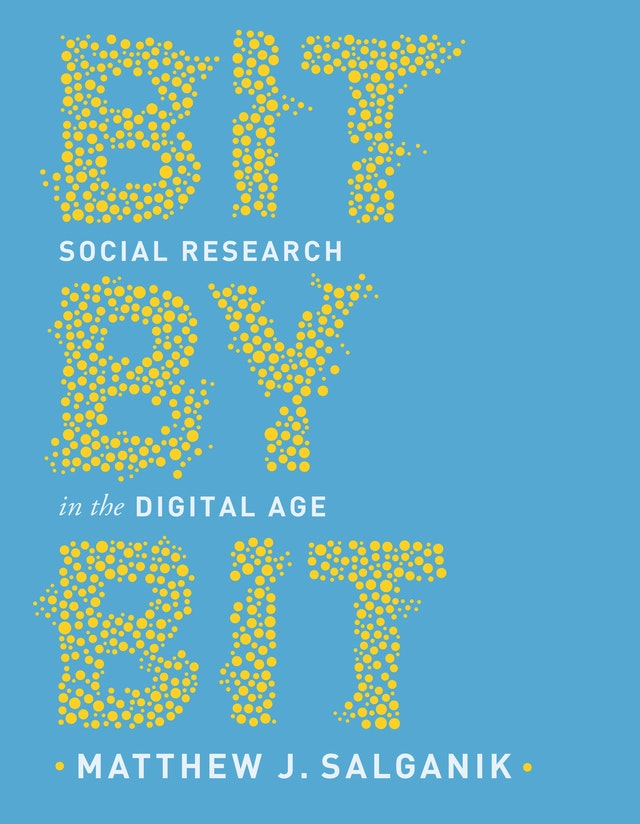
\includegraphics[width=\textwidth]{figures/salganik_bit_2018_cover}
\end{column}%

\hfill%

\begin{column}{.60\textwidth}
1) Introduction \\
2) Observing behavior \\
3) Asking questions \\
4) Running experiments \\
5) Mass collaboration \\
\textcolor{blue}{6) Ethics} \\
Part 1, Part 2, \textcolor{blue}{Additions and extensions} \\
7) The future \\
\end{column}%
\end{columns}

\end{frame}
%%%%%%%%%%%%%%%%%%%%%%%%%%
\begin{frame}

Ethics, part 1 and part 2
\begin{itemize}
\item Introduction
\item Three examples
\item Digital is different
\item Four principles
\item Two ethics frameworks
\item Four areas of difficulty
\item Practical tips
\end{itemize}

\end{frame}
%%%%%%%%%%%%%%%%%%%%%%%%%%
\begin{frame}

\begin{center}
Addition and extension 1 of 5: Respect for Law and Public Interest
\end{center}

\end{frame}
%%%%%%%%%%%%%%%%%%%%%%%%%
\begin{frame}

Four principles:
\begin{itemize}
\item Respect for persons
\item Beneficence
\item Justice
\item \textcolor{blue}{Respect for Law and Public Interest}
\end{itemize}

\end{frame}
%%%%%%%%%%%%%%%%%%%%%%%%%
\begin{frame}

Terms-of-service agreements

\end{frame}
%%%%%%%%%%%%%%%%%%%%%%%%%
\begin{frame}

\begin{center}
\includegraphics[width=0.9\textwidth]{figures/soeller_mapwatch_2016_title.png}
\end{center}

\vfill
\url{http://dx.doi.org/10.1145/2872427.2883016}
\end{frame}
%%%%%%%%%%%%%%%%%%%%%%%%%
\begin{frame}

Abstract:\\
``Maps have long played a crucial role in enabling people to conceptualize and navigate the world around them. However, maps also encode the world-views of their creators. Disputed international borders are one example of this: governments may mandate that cartographers produce maps that conform to their view of a territorial dispute. Today, online maps maintained by private corporations have become the norm. However, these new maps are still subject to old debates. Companies like Google and Bing resolve these disputes by localizing their maps to meet government requirements and user preferences, i.e., users in different locations are shown maps with different international boundaries. We argue that this non-transparent personalization of maps may exacerbate nationalistic disputes by promoting divergent views of geopolitical realities.''

\end{frame}
%%%%%%%%%%%%%%%%%%%%%%%
\begin{frame}

Abstract, part 2:\\
``To address this problem, we present MapWatch, our system for detecting and cataloging personalization of international borders in online maps. Our system continuously crawls all map tiles from Google and Bing maps, and leverages crowdworkers to identify border personalization. In this paper, we present the architecture of MapWatch, and analyze the instances of border personalization on Google and Bing, including one border change that MapWatch identified live, as Google was rolling out the update.''

\end{frame}
%%%%%%%%%%%%%%%%%%%%%%%%%
\begin{frame}

\begin{center}
\includegraphics[width=\textwidth]{figures/soeller_mapwatch_2016_fig5.png}
\end{center}

\vfill
\url{http://dx.doi.org/10.1145/2872427.2883016}
\end{frame}
%%%%%%%%%%%%%%%%%%%%%%%%%
\begin{frame}

\begin{center}
\includegraphics[width=\textwidth]{figures/soeller_mapwatch_2016_ethics.png}
\end{center}

\vfill
\url{http://dx.doi.org/10.1145/2872427.2883016}
\end{frame}
%%%%%%%%%%%%%%%%%%%%%%%%%
\begin{frame}

Researchers (with the support of the ACLU) have filed a case challenging the CFAA, Sandivg v Lynch:\\
\tiny{\textcolor{blue}{\url{https://www.aclu.org/cases/sandvig-v-lynch-challenge-cfaa-prohibition-uncovering-racial-discrimination-online}}}

\end{frame}
%%%%%%%%%%%%%%%%%%%%%%%%%%
\begin{frame}

Even if this is legal should we do it? \pause

Deen Freelon at SICSS 2018: ``\textcolor{blue}{\href{https://www.youtube.com/watch?v=GWpCHh54pXU}{Surviving the post-API age}}''

\begin{center}
\includegraphics[width=0.5\textwidth]{figures/freelon_postapi_screengrab}
\end{center}


If you go ``off the grid'': \pause
\begin{itemize}
\item you might lose access during your research
\pause
\item you might struggle to have your research funded, talk about it, and publish it
\pause
\item you might not be able to share your data with other researchers
\pause
\item you might make it harder to other academics in the future
\end{itemize}

\end{frame}
%%%%%%%%%%%%%%%%%%%%%%%%%%%
\begin{frame}

\begin{center}
Addition and extension 2 of 5: Informational risk
\end{center}

\end{frame}
%%%%%%%%%%%%%%%%%%%%%%%%%%%
\begin{frame}

Areas of difficulty:
\begin{enumerate}
\item Informed consent
\item \textcolor{blue}{Informational risk}
\item Privacy
\item Making decisions in the face of uncertainty
\end{enumerate}

\end{frame}
%%%%%%%%%%%%%%%%%%%%%%%%%%%
\begin{frame}

\begin{itemize}
\item \onslide<1>{Simple idea: Data can be made anonymous, and we can tell what data is sensitive}
\item \onslide<2>{\sout{Simple idea: Data can be made anonymous, and we can tell what data is sensitive}}
\item \onslide<2>{Better idea: All data are potentially identifiable and all data are potentially sensitive}
\end{itemize}

\end{frame}
%%%%%%%%%%%%%%%%%%%%%%%%%%%
\begin{frame}

\begin{center}
\only<1>{\includegraphics[width=\textwidth]{figures/re-identifcation-1}}
\only<2>{\includegraphics[width=\textwidth]{figures/re-identifcation-2}}
\only<3>{\includegraphics[width=\textwidth]{figures/re-identified}}
\end{center}

\vfill
\href{http://dx.doi.org/10.1142/S0218488502001648}{Sweeney (2002)}

\end{frame}
%%%%%%%%%%%%%%%%%%%%%%%%%%%
\begin{frame}

\begin{center}
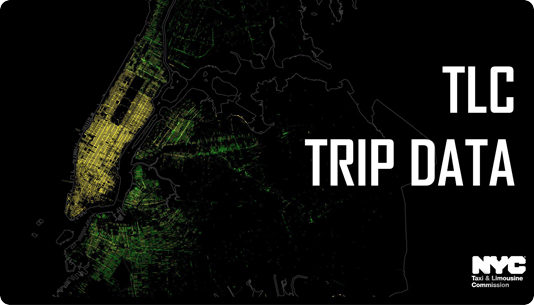
\includegraphics[width=\textwidth]{figures/nyc_taxi_data}
\end{center}

\end{frame}
%%%%%%%%%%%%%%%%%%%%%%
\begin{frame}

\begin{center}
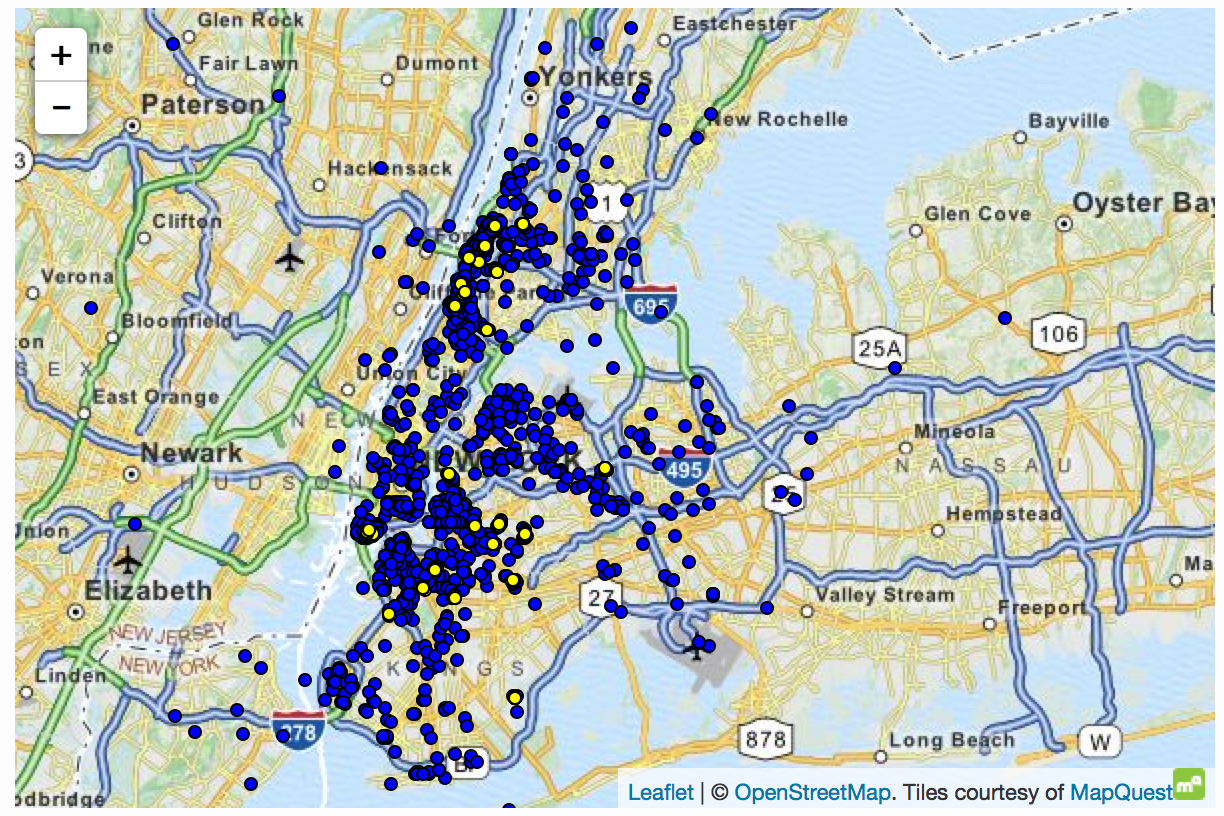
\includegraphics[width=1.1\textwidth]{figures/hustler_dropoff_wide.png}
\end{center}

\tiny{\url{http://research.neustar.biz/2014/09/15/riding-with-the-stars-passenger-privacy-in-the-nyc-taxicab-dataset/}}
\end{frame}
%%%%%%%%%%%%%%%%%%%%%%
\begin{frame}

\begin{center}
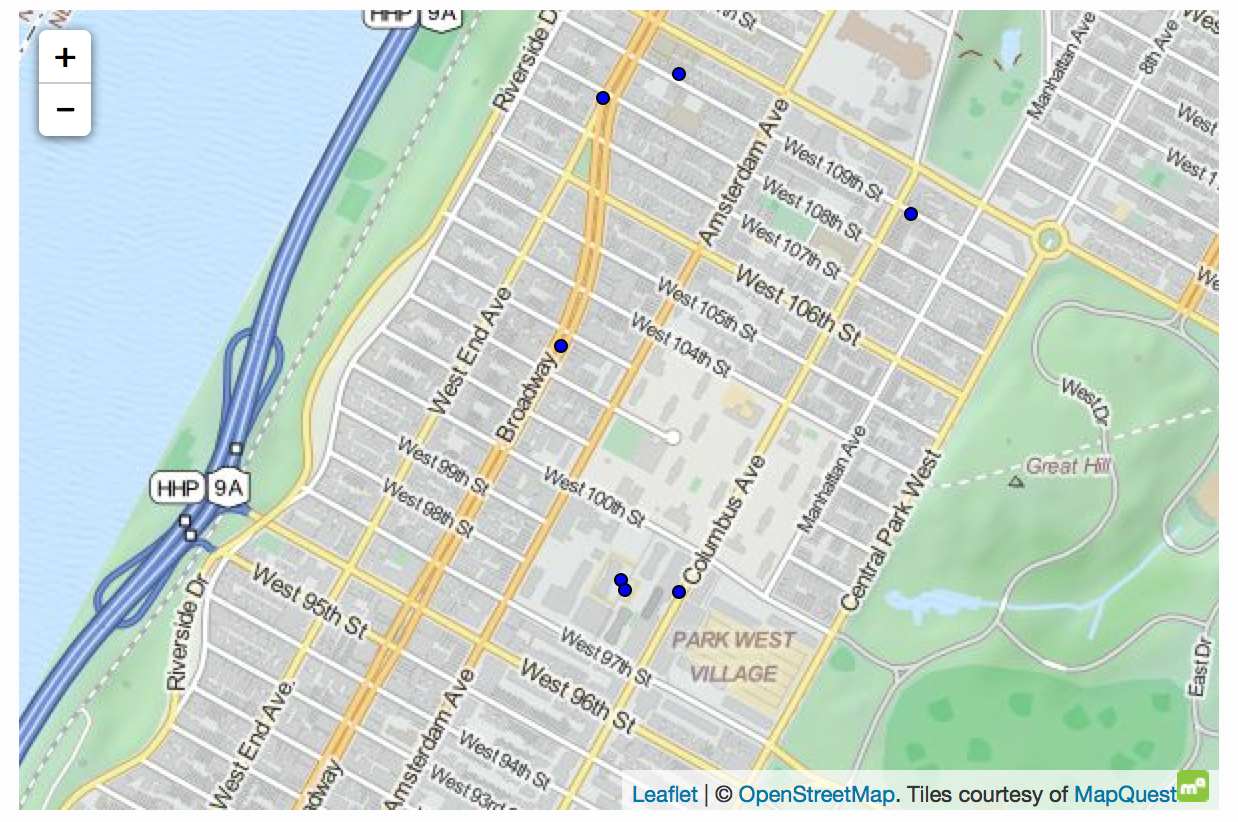
\includegraphics[width=\textwidth]{figures/hustler_dropoff_uws.png}
\end{center}

\tiny{\url{http://research.neustar.biz/2014/09/15/riding-with-the-stars-passenger-privacy-in-the-nyc-taxicab-dataset/}}
\end{frame}
%%%%%%%%%%%%%%%%%%%%%%
\begin{frame}[fragile]

Data:\\
\url{https://www1.nyc.gov/site/tlc/about/tlc-trip-record-data.page}
\pause

\vfill
Code:\\
\begin{tiny}
\begin{lstlisting} 
SELECT dropoff_latitude, dropoff_longitude
FROM tripData
WHERE pickup_lat > 40.767249 AND pickup_lat < 40.768
  AND pickup_lon > -73.996782 AND pickup_lon < -73.995538
  AND HOUR(pickup_datetime) < 6
  AND trip_distance > 5;
\end{lstlisting}
\end{tiny}

\end{frame}
%%%%%%%%%%%%%%%%%%%%%%
\begin{frame}

\begin{center}

\includegraphics[width=\textwidth]{figures/aol_search}
\end{center}

\end{frame}
%%%%%%%%%%%%%%%%%%%%%%
\begin{frame}

4417749, ``numb fingers'' \\ \pause
4417749, ``60 single men'' \\ \pause
4417749, ``dog that urinates on everything'' \\ \pause
4417749, ``landscapers in Lilburn, Ga'' \\ \pause
4417749,  [several people with the last name Arnold] \\ \pause
4417749,``homes sold in shadow lake subdivision gwinnett county georgia''\\

\end{frame}
%%%%%%%%%%%%%%%%%%%%%%
\begin{frame}

\begin{center}
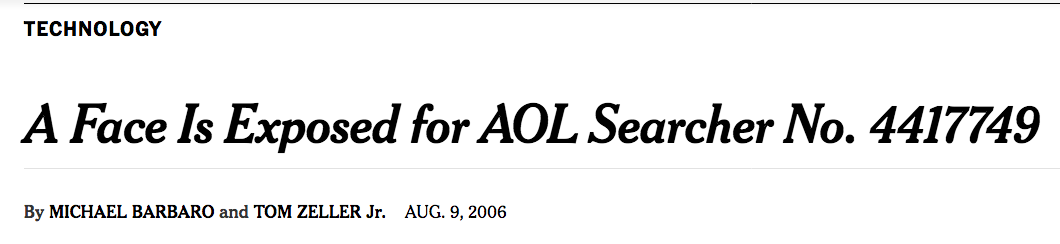
\includegraphics[width=\textwidth]{figures/barbaro_face_2006_title}
\end{center}

\vfill

\tiny{\url{https://www.nytimes.com/2006/08/09/technology/09aol.html}}

\end{frame}
%%%%%%%%%%%%%%%%%%%%%%%%%%
\begin{frame}

\begin{center}
Addition and extension 3 of 5: Fifth area of difficulty
\end{center}

\end{frame}
%%%%%%%%%%%%%%%%%%%%%%%%%%%
\begin{frame}

Areas of difficulty:
\begin{enumerate}
\item Informed consent
\item Informational risk
\item Privacy
\item Making decisions in the face of uncertainty
\pause 
\item Unanticipated secondary uses
\end{enumerate}

\end{frame}
%%%%%%%%%%%%%%%%%%%%%%%%%%%
\begin{frame}

\begin{center}
\includegraphics[width=\textwidth]{figures/ebird_screenshot}
\end{center}

\end{frame}
%%%%%%%%%%%%%%%%%%%%%%%%%%%
\begin{frame}

\begin{center}
\includegraphics[width=0.8\textwidth]{figures/glaser_plants_2019_title}
\end{center}

\vfill
\url{https://slate.com/technology/2019/04/superbloom-california-nature-internet-collide-birds-poaching-science.html}
\end{frame}
%%%%%%%%%%%%%%%%%%%%%%%%%%%
\begin{frame}

\begin{center}
\includegraphics[width=\textwidth]{figures/ebird_sensitive_species}
\end{center}

\vfill
\url{https://help.ebird.org/customer/en/portal/articles/2885265-sensitive-species-in-ebird}
\end{frame}
%%%%%%%%%%%%%%%%%%%%%%%%%%
\begin{frame}

\begin{center}
\includegraphics[width=0.4\textwidth]{figures/lex_luthor}
\end{center}

\begin{itemize}
\item How would Lex Luthor use this?
\item This requires adversarial thinking.
\end{itemize}

\vfill
\TINY{\url{https://en.wikipedia.org/wiki/Lex_Luthor\#/media/File:LexLuthor1.png}}

\end{frame}
%%%%%%%%%%%%%%%%%%%%%%%%%%%
\begin{frame}

\begin{center}
Addition and extension 4 of 5: Practical tips
\end{center}

\end{frame}
%%%%%%%%%%%%%%%%%%%%%%%%%
\begin{frame}

Practical tips:
\begin{itemize}
\item IRB is a floor not a ceiling
\item Put yourself in everyone else's shoes
\item Think of research ethics as continuous not discrete
\pause
\item Think of ethics as a research opportunity
\end{itemize}

\end{frame}
%%%%%%%%%%%%%%%%%%%%%%%%%%%
\begin{frame}

\begin{center}

\includegraphics[width=\textwidth]{figures/facct_star}
\end{center}

\vfill
\url{https://facctconference.org/}
\end{frame}
%%%%%%%%%%%%%%%%%%%%%%%%%%%
\begin{frame}

\begin{center}
Addition and extension 5 of 5: Think of ethics as a research opportunity, case study
\end{center}

\end{frame}
%%%%%%%%%%%%%%%%%%%%%%%%%
\begin{frame}

\begin{center}

\includegraphics[width=\textwidth]{figures/lundberg_privacy_2019_title}
\end{center}

\vfill
In press at \textit{Socius}, pre-print: \url{https://arxiv.org/abs/1809.00103}

\end{frame}
%%%%%%%%%%%%%%%%%%%%%%%%%
\begin{frame}

``Stewards of social science data face a fundamental tension. On one hand, they want to make their data accessible to as many researchers as possible to facilitate new discoveries. At the same time, they want to restrict access to their data as much as possible in order to protect the people represented in the data. In this paper, we provide a case study addressing this common tension in an uncommon setting: the Fragile Families Challenge, a scientific mass collaboration designed to yield insights that could improve the lives of disadvantaged children in the United States. We describe our process of threat modeling, threat mitigation, and third-party guidance. We also describe the ethical principles that formed the basis of our process. We are open about our process and the trade-offs that we made in the hopes that others can improve on what we have done.''

\vfill
In press at \textit{Socius}, pre-print: \url{https://arxiv.org/abs/1809.00103}
\end{frame}
%%%%%%%%%%%%%%%%%%%%%%%%%
\begin{frame}

Ethics, part 1 and part 2
\begin{itemize}
\item Introduction
\item Three examples
\item Digital is different
\item Four principles
\item Two ethics frameworks
\item Four areas of difficulty
\item Practical tips
\end{itemize}

\end{frame}
%%%%%%%%%%%%%%%%%%%%%%%%
\begin{frame}

Additions and extensions
\begin{itemize}
\item 1 of 5: Respect for Law and Public Interest
\item 2 of 5: Informational risk
\item 3 of 5: Fifth area of difficulty
\item 4 of 5: Practical tips
\item 5 of 5: Think of ethics as a research opportunity, case study
\end{itemize}

\end{frame}
%%%%%%%%%%%%%%%%%%%%%%%%
\begin{frame}

\begin{center}
\Large Thank you
\end{center}

\end{frame}
%%%%%%%%%%%%%%%%%%%%%%%%


\end{document}

